\documentclass[aspectratio=169,11pt]{beamer}
\usetheme{default}
\usefonttheme{serif}
\setbeamertemplate{navigation symbols}{}
\setbeamertemplate{footline}[frame number]
\setbeamertemplate{itemize items}[circle]
\setbeamersize{text margin left=10mm,text margin right=10mm}
\usepackage{fontspec}
\usepackage{unicode-math}
\setmainfont{STIX2Text}[Path=fonts/, Extension=.otf,
  UprightFont=*-Regular, ItalicFont=*-Italic,
  BoldFont=*-Bold, BoldItalicFont=*-BoldItalic]
\setmathfont{STIX2Math}[Path=fonts/, Extension=.otf]
\usepackage{booktabs}
\usepackage{tikz}
\usetikzlibrary{arrows.meta,positioning,calc}
\definecolor{arb}{RGB}{27,94,52}
\definecolor{arbred}{RGB}{150,40,40}
\definecolor{arbdim}{RGB}{100,100,100}
\setbeamercolor{structure}{fg=arb}
\setbeamercolor{frametitle}{fg=arb}
\setbeamercolor{alerted text}{fg=arbred}
\setbeamerfont{frametitle}{size=\Large,series=\bfseries}
\setbeamerfont{title}{size=\huge,series=\bfseries}

\newcommand{\F}{\mathbb{F}}
\newcommand{\G}{\mathbb{G}}
\newcommand{\Ep}{\ensuremath{\mathcal{E}}}
\newcommand{\Pallas}{\ensuremath{\mathsf{Pallas}}}
\newcommand{\Vesta}{\ensuremath{\mathsf{Vesta}}}
\newcommand{\Fpp}{\ensuremath{\F_{p}}}
\newcommand{\nfsym}{\ensuremath{\mathsf{nf}}}
\newcommand{\cmsym}{\ensuremath{\mathsf{cm}}}
\newcommand{\cmx}{\ensuremath{\mathsf{cmx}}}
\newcommand{\cvsym}{\ensuremath{\mathsf{cv}}}
\newcommand{\rksym}{\ensuremath{\mathsf{rk}}}
\newcommand{\gd}{\ensuremath{\mathsf{g_d}}}
\newcommand{\pkd}{\ensuremath{\mathsf{pk_d}}}
\newcommand{\aksym}{\ensuremath{\mathsf{ak}}}
\newcommand{\nksym}{\ensuremath{\mathsf{nk}}}
\newcommand{\asksym}{\ensuremath{\mathsf{ask}}}
\newcommand{\ivk}{\ensuremath{\mathsf{ivk}}}
\newcommand{\fvk}{\ensuremath{\mathsf{fvk}}}
\newcommand{\ovk}{\ensuremath{\mathsf{ovk}}}
\newcommand{\dk}{\ensuremath{\mathsf{dk}}}
\newcommand{\rcm}{\ensuremath{\mathsf{rcm}}}
\newcommand{\rcv}{\ensuremath{\mathsf{rcv}}}
\newcommand{\rivk}{\ensuremath{\mathsf{r_{ivk}}}}
\newcommand{\rsk}{\ensuremath{\mathsf{rsk}}}
\newcommand{\esk}{\ensuremath{\mathsf{esk}}}
\newcommand{\epk}{\ensuremath{\mathsf{epk}}}
\newcommand{\Extract}{\ensuremath{\mathsf{Extract}}}
\newcommand{\NoteCommit}{\ensuremath{\mathsf{NoteCommit}}}
\newcommand{\GroupHash}{\ensuremath{\mathsf{GroupHash}}}
\newcommand{\CommitIvk}{\ensuremath{\mathsf{Commit}^{\mathsf{ivk}}}}
\newcommand{\ip}[2]{\langle #1,\, #2 \rangle}
\newcommand{\bvk}{\ensuremath{\mathsf{bvk}}}
\newcommand{\bsk}{\ensuremath{\mathsf{bsk}}}
\newcommand{\vbal}{\ensuremath{v_{\mathrm{balance}}}}
\newcommand{\Ecenc}{\ensuremath{C_{\mathrm{enc}}}}
\newcommand{\Ecout}{\ensuremath{C_{\mathrm{out}}}}
\newcommand{\Ecv}{\ensuremath{\cvsym}}
\newcommand{\Enf}{\ensuremath{\nfsym}}
\newcommand{\Eanc}{\ensuremath{\mathsf{anchor}}}
\newcommand{\Dint}[1]{\ensuremath{#1^{\mathsf{int}}}}
\newcommand{\Dprf}[1]{\ensuremath{\mathsf{PRFexpand}_{#1}}}
\newcommand{\Dff}{\ensuremath{\mathsf{FF1}}}
\newcommand{\GZH}{\ensuremath{Z_H}}
\newcommand{\Glo}[1]{\ensuremath{#1_{\mathrm{lo}}}}
\newcommand{\Ghi}[1]{\ensuremath{#1_{\mathrm{hi}}}}

\newcommand{\divider}[1]{\begin{frame}[plain]\vfill\centering
  {\usebeamercolor[fg]{structure}\Huge\bfseries #1}\vfill\end{frame}}
\newcommand{\grey}[1]{{\color{arbdim}#1}}

% ---- The commitment tree (depth 3 toy; the real tree has depth 32).
\newcommand{\CTreeMode}{none}
\newcommand{\CTreeAnchor}{anchor}
\newcommand{\CTreeLeaf}{leaf}
\newcommand{\CTreePath}{path}
\newcommand{\TreeFig}[1][none]{%
  \renewcommand{\CTreeMode}{#1}%
  \tikzset{croot/.style={},cleaf/.style={},croute/.style={},
    csib/.style={},cedge/.style={}}%
  \ifx\CTreeMode\CTreeAnchor\tikzset{croot/.style={chl}}\fi
  \ifx\CTreeMode\CTreeLeaf\tikzset{cleaf/.style={chl}}\fi
  \ifx\CTreeMode\CTreePath\tikzset{cleaf/.style={chl},croute/.style={chl},
    csib/.style={fill=arb!25},cedge/.style={draw=arbred,very thick}}\fi
  \begin{tikzpicture}[x=7.2mm,y=7.5mm,every node/.style={font=\scriptsize},
    lf/.style={draw,minimum width=6mm,minimum height=4mm,inner sep=1pt},
    nd/.style={draw,circle,inner sep=1.6pt},
    ed/.style={black!55},
    chl/.style={draw=arbred,very thick,fill=arbred!15}]
  \node[lf] (L0) at (0,0) {\cmx};
  \node[lf] (L1) at (1,0) {\cmx};
  \node[lf,cleaf] (L2) at (2,0) {\cmx};
  \node[lf,csib] (L3) at (3,0) {\cmx};
  \node[lf] (L4) at (4,0) {\cmx};
  \node[lf] (L5) at (5,0) {\cmx};
  \node[lf] (L6) at (6,0) {\cmx};
  \node[lf,dashed] (L7) at (7,0) {$\varnothing$};
  \node[nd,csib] (A) at (0.5,1) {};
  \node[nd,croute] (B) at (2.5,1) {};
  \node[nd] (C) at (4.5,1) {};
  \node[nd] (D) at (6.5,1) {};
  \node[nd,croute] (E) at (1.5,2) {};
  \node[nd,csib] (F) at (5.5,2) {};
  \node[draw,rounded corners,fill=arb!15,croot] (R) at (3.5,3) {anchor};
  \draw[ed] (A)--(L0); \draw[ed] (A)--(L1); \draw[ed] (B)--(L3);
  \draw[ed] (C)--(L4); \draw[ed] (C)--(L5); \draw[ed] (D)--(L6);
  \draw[ed] (D)--(L7); \draw[ed] (E)--(A); \draw[ed] (F)--(C);
  \draw[ed] (F)--(D); \draw[ed] (R)--(F);
  \draw[ed,cedge] (L2)--(B); \draw[ed,cedge] (B)--(E);
  \draw[ed,cedge] (E)--(R);
  \ifx\CTreeMode\CTreeLeaf
    \node[text=arbred,below=1pt of L2] {$p$};\fi
  \ifx\CTreeMode\CTreePath
    \node[text=arbred,below=1pt of L2] {$p$};\fi
  \end{tikzpicture}}

% ---- The key ladder.
\newcommand{\LadderFig}{%
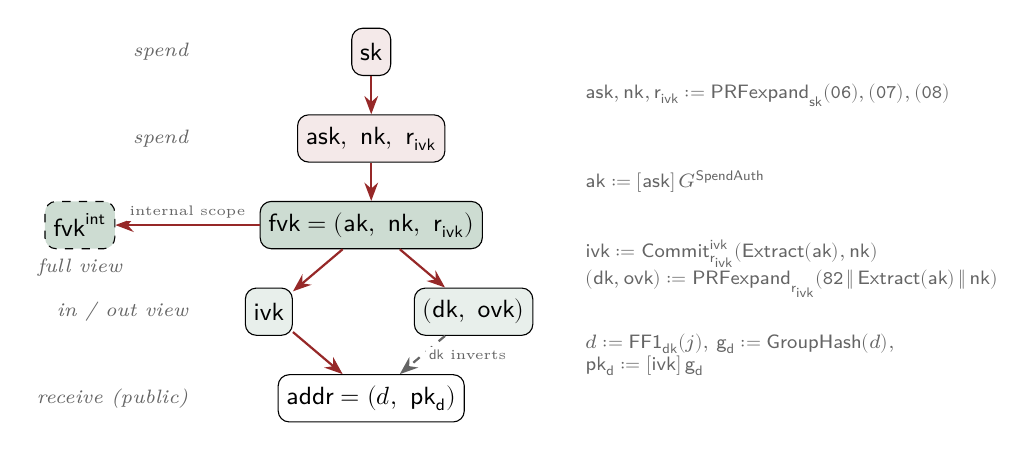
\begin{tikzpicture}[font=\small, x=1cm, y=1cm,
  k/.style={draw, rounded corners, inner sep=3pt, minimum height=6mm,
            anchor=center, fill=arb!10},
  kspend/.style={k, fill=arbred!10},
  kfull/.style={k, fill=arb!22},
  kpub/.style={k, fill=white},
  kint/.style={k, dashed, fill=arb!22},
  tier/.style={font=\scriptsize\itshape, text=arbdim, anchor=east},
  op/.style={font=\scriptsize, text=arbdim, anchor=west, align=left},
  elab/.style={font=\tiny, text=arbdim, inner sep=1pt, fill=white},
  ow/.style={-{Stealth}, thick, arbred},
  inv/.style={-{Stealth}, thick, arbdim, dashed}]
\node[kspend] (sk)    at (0,0)       {$\mathsf{sk}$};
\node[kspend] (mid)   at (0,-1.1)    {$\asksym,\ \nksym,\ \rivk$};
\node[kfull]  (fvk)   at (0,-2.2)    {$\fvk = (\aksym,\ \nksym,\ \rivk)$};
\node[kint]   (int)   at (-3.7,-2.2) {$\Dint{\fvk}$};
\node[k]      (ivk)   at (-1.3,-3.3) {$\ivk$};
\node[k]      (dkovk) at (1.3,-3.3)  {$(\dk,\ \ovk)$};
\node[kpub]   (addr)  at (0,-4.4)    {$\mathsf{addr} = (d,\ \pkd)$};
\draw[ow] (sk)  -- (mid);
\draw[ow] (mid) -- (fvk);
\draw[ow] (fvk) -- (ivk);
\draw[ow] (fvk) -- (dkovk);
\draw[ow] (fvk) -- node[elab, above=1pt]{internal scope} (int);
\draw[ow] (ivk) -- (addr);
\draw[inv] (dkovk) -- node[elab, right=1pt]{$\dk$ inverts} (addr);
\node[op] at (2.6,-0.55)
  {$\asksym, \nksym, \rivk := \Dprf{\mathsf{sk}}(\mathtt{06}), (\mathtt{07}), (\mathtt{08})$};
\node[op] at (2.6,-1.65)
  {$\aksym := [\asksym]\,G^{\mathsf{SpendAuth}}$};
\node[op] at (2.6,-2.75)
  {$\ivk := \CommitIvk_{\rivk}(\Extract(\aksym), \nksym)$\\
   $(\dk, \ovk) := \Dprf{\rivk}(\mathtt{82}\,\|\,\Extract(\aksym)\,\|\,\nksym)$};
\node[op] at (2.6,-3.85)
  {$d := \Dff_{\dk}(j)$, $\gd := \GroupHash(d)$,\\
   $\pkd := [\ivk]\,\gd$};
\node[tier] at (-2.2,0)    {spend};
\node[tier] at (-2.2,-1.1) {spend};
\node[tier, anchor=north] at (int.south) {full view};
\node[tier] at (-2.2,-3.3) {in / out view};
\node[tier] at (-2.2,-4.4) {receive (public)};
\end{tikzpicture}}

% ---- One Action inside its bundle.
\newcommand{\ActionBox}[1][none]{%
  \tikzset{hlnone/.style={}, hlanchor/.style={}, hlnf/.style={},
    hlcv/.style={}, hlrk/.style={}, hlcmx/.style={}, hlproof/.style={},
    hl#1/.style={draw=arbred, very thick, fill=arbred!15}}%
  \begin{tikzpicture}[font=\scriptsize, x=1cm, y=1cm,
    ebox/.style={draw=black!60, fill=white, rounded corners=2pt,
      inner sep=2.5pt, align=center},
    elab/.style={inner sep=2pt, text=black!60}]
  \draw[draw=black!50, dashed, rounded corners=3pt]
    (-2.45,-2.45) rectangle (4.75,2.5);
  \node[elab, anchor=north west, text=black!70, font=\scriptsize\bfseries]
    at (-2.45,2.5) {bundle};
  \draw[draw=arb!40, rounded corners=3pt] (-2.0,-2.1) rectangle (2.4,2.1);
  \node[elab, anchor=south east, text=arb!60] at (2.4,2.1) {$\times\,n$};
  \node[draw=arb, thick, fill=white, rounded corners=3pt,
    minimum width=4.4cm, minimum height=3.9cm] (act) at (0,0) {};
  \node[anchor=north west, font=\scriptsize\bfseries, text=arb,
    inner sep=2pt] at (act.north west) {Action};
  \node[draw=arb!60, fill=arb!8, rounded corners=2pt, inner sep=3pt,
    align=center, anchor=north, text width=3.8cm] (wit) at (0,1.62)
    {\textbf{witness} --- never published\\
     old note, new note\\
     Merkle path $+$ position\\
     $\aksym, \nksym, \rivk, \ivk$; $\alpha$, $\rcv$};
  \node[elab, anchor=west] at (-2.15,-0.12) {public, per Action};
  \node[ebox, hlcv, anchor=west] (cv) at (-2.05,-0.58) {$\Ecv$};
  \node[ebox, hlnf, right=1.2mm of cv] (nf) {$\Enf$};
  \node[ebox, hlrk, right=1.2mm of nf] (rk) {$\rksym$};
  \node[ebox, hlcmx, right=1.2mm of rk] (cmx) {$\cmx$};
  \node[ebox, draw=black!40, dashed] (ct) at (0,-1.15)
    {$\epk,\ \Ecenc,\ \Ecout$};
  \node[elab, align=center, font=\tiny, text=black!60] at (0,-1.66)
    {delivery ciphertexts --- opened only with $\ivk$ / $\ovk$};
  \node[ebox, hlanchor, anchor=west] (anc) at (2.45,1.65) {$\Eanc$};
  \node[ebox, anchor=west] (flg) at (2.45,1.0) {flags};
  \node[ebox, anchor=west] (vb)  at (2.45,0.35) {$\vbal$};
  \node[ebox, hlproof, anchor=west] (prf) at (2.45,-0.3) {proof};
  \node[ebox, anchor=west] (sas) at (2.45,-0.95) {SpendAuthSigs};
  \node[ebox, anchor=west] (bsg) at (2.45,-1.6) {binding sig};
  \end{tikzpicture}}

% ---- The deficit walk: two seeded runs from z = 2.
\newcommand{\Kwalk}{%
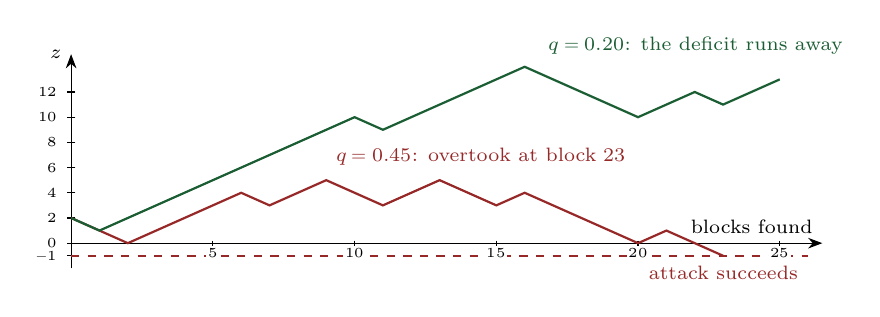
\begin{tikzpicture}[x=0.36cm, y=0.16cm]
\draw[-{Stealth[length=1.8mm]}] (0,-2) -- (0,15)
  node[left, font=\scriptsize] {$z$};
\draw[-{Stealth[length=1.8mm]}] (0,0) -- (26.5,0)
  node[above left, font=\scriptsize] {blocks found};
\foreach \y in {-1, 0, 2, 4, 6, 8, 10, 12}
  \draw (0.15,\y) -- (-0.15,\y) node[left, font=\tiny] {$\y$};
\draw[dashed, thick, arbred] (0,-1) -- (26,-1)
  node[below left, font=\scriptsize, text=arbred] {attack succeeds};
\foreach \x in {5, 10, 15, 20, 25}
  \draw (\x,0.2) -- (\x,-0.2) node[below, font=\tiny, fill=white,
    inner sep=0.6pt] {$\x$};
\draw[thick, arbred] plot coordinates {(0,2) (1,1) (2,0) (3,1) (4,2)
  (5,3) (6,4) (7,3) (8,4) (9,5) (10,4) (11,3) (12,4) (13,5) (14,4)
  (15,3) (16,4) (17,3) (18,2) (19,1) (20,0) (21,1) (22,0) (23,-1)};
\node[font=\scriptsize, text=arbred, anchor=south west] at (9,5.4)
  {$q = 0.45$: overtook at block $23$};
\draw[thick, arb] plot coordinates {(0,2) (1,1) (2,2) (3,3) (4,4) (5,5)
  (6,6) (7,7) (8,8) (9,9) (10,10) (11,9) (12,10) (13,11) (14,12) (15,13)
  (16,14) (17,13) (18,12) (19,11) (20,10) (21,11) (22,12) (23,11)
  (24,12) (25,13)};
\node[font=\scriptsize, text=arb, anchor=south west] at (16.5,14.2)
  {$q = 0.20$: the deficit runs away};
\end{tikzpicture}}

% ---- A sigma protocol, three moves.
\newcommand{\SigmaFig}[3]{%
\begin{tikzpicture}[x=1cm,y=1cm,font=\small,
  who/.style={font=\small\bfseries,text=arb},
  msg/.style={-{Stealth[length=2mm]},thick}]
\node[who] (P) at (0,0) {Prover};
\node[who] (V) at (7,0) {Verifier};
\draw[black!30] (0,-0.35) -- (0,-3.6);
\draw[black!30] (7,-0.35) -- (7,-3.6);
\draw[msg] (0.2,-1.0) -- (6.8,-1.0) node[midway,above] {#1};
\draw[msg] (6.8,-2.0) -- (0.2,-2.0) node[midway,above] {#2};
\draw[msg] (0.2,-3.0) -- (6.8,-3.0) node[midway,above] {#3};
\end{tikzpicture}}

\title{Ironwood, the core}
\subtitle{how Zcash verifies a shielded transfer without seeing it}
\author{m@rek.onl}
\date{}

\begin{document}

\begin{frame}[plain]
\titlepage
\end{frame}

% ====================================================================
\begin{frame}{What a validator checks}
\Large
\begin{enumerate}\itemsep8pt
  \item the coin \textbf{exists} \grey{--- look it up}
  \item the spend is \textbf{authorised} \grey{--- script and signature}
  \item it is not spent \textbf{twice} \grey{--- delete it}
  \item value is \textbf{conserved} \grey{--- $\sum\mathrm{in} \ge \sum\mathrm{out}$}
\end{enumerate}
\vfill
\normalsize
Every check reads the transaction in the clear: which coin, whose key,
how much.
\end{frame}

\begin{frame}{Privacy, precisely}
Hide the sender, the receiver and the amount --- while a stranger still
runs all four checks.
\vfill
\begin{center}
\begin{tabular}{@{}ll@{}}
\toprule
check & mechanism \\
\midrule
exists & a commitment in a Merkle tree, membership proved in zero knowledge \\
not twice & a nullifier: a keyed serial number, revealed once \\
conserved & homomorphic value commitments and a binding signature \\
authorised & a proof of key knowledge and a re-randomised signature \\
\bottomrule
\end{tabular}
\end{center}
\vfill
One zero-knowledge statement per Action carries all four; one proof per bundle.
\end{frame}

% ====================================================================
\divider{Anchors}

\begin{frame}{A group and a hard problem}
\[
\Ep(\Fpp):\quad y^2 = x^3 + 5 \quad\text{over } \Fpp,\qquad
p \approx 2^{254},\quad |\Ep| = q \text{ prime}
\]
\[
[a]\,G := \underbrace{G + G + \cdots + G}_{a\ \text{times}}
\qquad\qquad
\text{given } G \text{ and } [a]\,G,\ \text{find } a:\ \text{infeasible}
\]
\vfill
\begin{itemize}
  \item Pallas: points over $\Fpp$, scalars in $\F_q$.
  \item Vesta: the same curve with $p$ and $q$ swapped --- a cycle.
  \item Everything below is built from $[a]\,G$ and the discrete log.
\end{itemize}
\end{frame}

\begin{frame}{Commitments}
\[
C(v, r) := [v]\,V + [r]\,R \qquad V, R \text{ independent points}
\]
\vfill
\begin{itemize}\itemsep6pt
  \item \textbf{Hiding:} $r$ uniform, so $C$ is a uniform point; $v$ is invisible.
  \item \textbf{Binding:} two openings $(v, r) \ne (v', r')$ of one $C$ give
    $\log_R V = (r' - r)/(v - v')$.
  \item \textbf{Homomorphic:} $C(v_1, r_1) + C(v_2, r_2) = C(v_1 + v_2,\ r_1 + r_2)$.
\end{itemize}
\vfill
A sealed envelope that can be added to other sealed envelopes.
\end{frame}

\begin{frame}{Hashes and Merkle trees}
\begin{columns}[c]
\begin{column}{0.5\textwidth}
\centering\TreeFig[path]
\end{column}
\begin{column}{0.46\textwidth}
\begin{itemize}\itemsep6pt
  \item Hash $\mathsf{H}$ collision resistant: nobody can find two inputs
    with one output.
  \item The root commits to every leaf.
  \item Membership of leaf $p$: its $32$ siblings, hashed upward, reach the root.
  \item Append only: old roots stay valid forever.
\end{itemize}
\end{column}
\end{columns}
\end{frame}

\begin{frame}{A sigma protocol: Schnorr identification}
Prover knows $x$ with $X = [x]\,G$.
\begin{center}
\SigmaFig{$R = [k]\,G$, \ $k$ random}{$c$ random}{$s = k + c\,x$}
\end{center}
\[
\text{Verifier checks}\qquad [s]\,G \overset{?}{=} R + [c]\,X
\]
\end{frame}

\begin{frame}{Why it proves, and why it hides}
\textbf{Special soundness.} Two accepting transcripts with the same $R$:
\[
(R, c, s),\ (R, c', s')\ \Longrightarrow\ x = \frac{s - s'}{c - c'}
\]
whoever answers two challenges knows $x$.
\vfill
\textbf{Zero knowledge.} A simulator with no $x$ picks $c$ and $s$ first:
\[
R := [s]\,G - [c]\,X
\]
the transcript has exactly the real distribution. The verifier learns
nothing it could not have made itself.
\end{frame}

\begin{frame}{Fiat--Shamir: the verifier becomes a hash}
\[
c := \mathsf{H}(X,\ R,\ m)
\]
\vfill
\begin{itemize}\itemsep6pt
  \item The prover cannot pick $R$ after $c$: $c$ depends on $R$.
  \item The pair $(R, s)$ is now a signature on $m$ --- Schnorr.
  \item \textbf{sigma protocol $+$ Fiat--Shamir $=$ Schnorr signature.}
  \item Zcash's RedPallas is Schnorr on Pallas, with one addition:
    the key can be re-randomised (later).
\end{itemize}
\end{frame}

\begin{frame}{Zero-knowledge proofs, in general}
A relation $\mathcal{R}(x, w)$: public statement $x$, private witness $w$.
\[
\mathsf{Prove}(x, w) \to \pi \qquad\qquad \mathsf{Verify}(x, \pi) \in \{0, 1\}
\]
\vfill
\begin{itemize}\itemsep6pt
  \item \textbf{Complete:} an honest $\pi$ verifies.
  \item \textbf{Knowledge sound:} from any convincing prover an extractor
    pulls a $w$ with $\mathcal{R}(x, w)$.
  \item \textbf{Zero knowledge:} a simulator given only $x$ reproduces $\pi$.
  \item \textbf{SNARK:} $\pi$ short (logarithmic) and non-interactive (Fiat--Shamir).
\end{itemize}
\vfill
Schnorr is the proof for $\mathcal{R} = \{(X, x) : X = [x]\,G\}$.
\end{frame}

\begin{frame}{A polynomial cannot lie everywhere}
\[
D \ne 0,\ \deg D \le d
\quad\Longrightarrow\quad
\Pr_{z \leftarrow \F}\bigl[D(z) = 0\bigr] \le \frac{d}{|\F|}
\]
\vfill
A nonzero polynomial has at most $d$ roots. Fix $D$ first, draw $z$
second: one random probe catches it.
\vfill
With $|\F| \approx 2^{254}$ and $d \approx 2^{14}$ the odds of escape are
about $2^{-240}$.
\end{frame}

% ====================================================================
\divider{The core of Orchard}

\begin{frame}{A note}
\[
n = (\,d,\ \pkd,\ v,\ \rho,\ \psi,\ \rcm\,)
\]
\[
\cmsym = \NoteCommit_{\rcm}(\gd,\ \pkd,\ v,\ \rho,\ \psi),
\qquad
\cmx = \Extract(\cmsym) \in \Fpp
\]
\vfill
\begin{tabular}{@{}ll@{}}
$(d, \pkd)$ & the recipient's diversified address \\
$v$ & the value, $0 \le v < 2^{64}$ \\
$\rho, \psi$ & uniqueness seed and nullifier salt \\
$\rcm$ & the commitment trapdoor \\
\end{tabular}
\vfill
On chain: $\cmx$ and a ciphertext. Nothing else about the note.
\end{frame}

\begin{frame}{The chain's shielded state}
\begin{columns}[c]
\begin{column}{0.5\textwidth}
\centering\TreeFig[anchor]
\end{column}
\begin{column}{0.46\textwidth}
\begin{itemize}\itemsep6pt
  \item \textbf{The commitment tree:} depth $32$, append only; every
    block's final root is an \emph{anchor}.
  \item \textbf{The nullifier set:} the spent half, growing; a nullifier
    names no leaf.
  \item A spend proves membership under some anchor and reveals a nullifier.
\end{itemize}
\end{column}
\end{columns}
\end{frame}

\begin{frame}{The nullifier}
\[
\nfsym := \Extract\bigl(\,[\,F_{\nksym}(\rho) + \psi\,]\,G^{\mathsf{nf}} + \cmsym\,\bigr)
\]
\vfill
\begin{itemize}\itemsep6pt
  \item Keyed by $\nksym$, the owner's nullifier key; $F_{\nksym}$ is
    Poseidon, a hash the circuit evaluates natively.
  \item Seeded by $\rho$, salted by $\psi$, bound to $\cmsym$.
  \item Chaining $\rho_{\mathrm{new}} := \nfsym_{\mathrm{old}}$: every note inherits
    the nullifier of the note spent beside it, so $\rho$ is unique.
  \item Unique, and unlinkable to $\cmsym$ without $\nksym$.
\end{itemize}
\end{frame}

\begin{frame}{Keys}
\centering
\LadderFig
\end{frame}

\begin{frame}{Diversified addresses}
\[
d \in \{0,1\}^{88},\qquad \gd := \GroupHash(d),\qquad \pkd := [\ivk]\,\gd
\]
\vfill
\begin{itemize}\itemsep6pt
  \item Some $2^{88}$ addresses per key, all paid into one wallet.
  \item Unlinkable to each other, even by the payer: two addresses share
    $\ivk$ only as a discrete log.
  \item One $\ivk$ detects every payment to every address.
\end{itemize}
\end{frame}

\begin{frame}{The Action}
\begin{columns}[c]
\begin{column}{0.56\textwidth}
\centering\ActionBox
\end{column}
\begin{column}{0.42\textwidth}
\begin{itemize}\itemsep6pt
  \item One Action spends one note and creates one note.
  \item A dummy note pads either side; every Action looks alike.
  \item One proof per bundle covers all its Actions.
\end{itemize}
\end{column}
\end{columns}
\end{frame}

\begin{frame}{The statement}
\begin{center}
\begin{tabular}{@{}lll@{}}
\toprule
check & clause & the proof establishes \\
\midrule
exists & A3 & a Merkle path from $\cmsym_{\mathrm{old}}$ to the anchor \\
not twice & A5 & the nullifier $\nfsym$ is this note's serial, keyed by $\nksym$ \\
conserved & A4 & the commitment $\cvsym$ hides $v_{\mathrm{old}} - v_{\mathrm{new}}$, both $< 2^{64}$ \\
authorised & A6, A7 & the key $\rksym$ disguises $\aksym$; $\aksym, \nksym$ sit behind the address \\
\addlinespace
well-formed & A1, A2 & both commitments open to notes; $\rho_{\mathrm{new}} = \nfsym_{\mathrm{old}}$ \\
gated & A8--A10 & spends, outputs, cross-address payments switched by flags \\
\bottomrule
\end{tabular}
\end{center}
\vfill
The witness: both notes, the path and position, the keys, $\alpha$, $\rcv$.\\
The one check the proof cannot make: has this $\nfsym$ been seen before.
\end{frame}

\begin{frame}{Conservation without amounts}
\[
\cvsym = [\,v_{\mathrm{old}} - v_{\mathrm{new}}\,]\,V + [\rcv]\,R
\qquad\text{per Action}
\]
\[
\bvk := \sum_i \cvsym_i - [\vbal]\,V
\;=\; [\,\textstyle\sum_i \rcv_i\,]\,R \quad\text{iff the books balance}
\]
\vfill
\begin{itemize}\itemsep6pt
  \item The balance $\vbal$ is public: the net flow out of the pool; for a fully
    shielded transfer, the fee.
  \item The binding signature is Schnorr under $\bvk$ on base $R$:
    knowing its secret key means knowing $\sum \rcv$, which exists only
    when the amounts cancel.
\end{itemize}
\end{frame}

\begin{frame}{Authorisation without a fixed key}
\[
\rksym := \aksym + [\alpha]\,G^{\mathsf{SpendAuth}},
\qquad
\rsk := \asksym + \alpha
\]
\vfill
\begin{itemize}\itemsep6pt
  \item One $\aksym$ per wallet; publishing it would stamp every spend.
  \item Fresh $\alpha$ per spend: $\rksym$ is a uniform point, unlinkable.
  \item The signature is Schnorr under $\rksym$; the circuit proves
    $\rksym$ was formed from the $\aksym$ behind the spent note's address.
\end{itemize}
\end{frame}

\begin{frame}{Delivery}
\[
\epk := [\esk]\,\gd,\qquad
\mathsf{s} := [\esk]\,\pkd = [\ivk]\,\epk,\qquad
K := \mathsf{KDF}(\mathsf{s}, \epk)
\]
\[
\Ecenc := \mathsf{AEAD}_K(\,\mathtt{0x03}, d, v, \mathsf{rseed}, \mathsf{memo}\,)
\]
\vfill
\begin{itemize}\itemsep6pt
  \item One-shot Diffie--Hellman to the diversified base, then
    ChaCha20-Poly1305.
  \item No address on chain: the recipient trial-decrypts every output
    with $\ivk$. A wrong key is rejected by the tag.
  \item The ciphertext $\Ecout$ is the sender's own copy, under $\ovk$.
\end{itemize}
\end{frame}

\begin{frame}{The doors}
\begin{center}
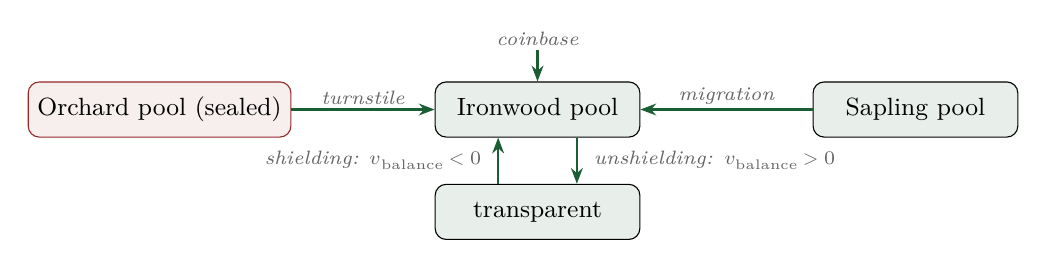
\begin{tikzpicture}[x=1mm,y=1mm,
  pool/.style={draw,rounded corners,minimum width=26mm,minimum height=7mm,
    fill=arb!10,font=\small},
  sealed/.style={pool,fill=arbred!8,draw=arbred},
  flow/.style={-{Stealth[length=2mm]},thick,arb},
  lbl/.style={font=\scriptsize\itshape,text=arbdim,inner sep=1.5pt}]
\node[sealed] (o) at (-48,0) {Orchard pool (sealed)};
\node[pool] (i) at (0,0) {Ironwood pool};
\node[pool] (s) at (48,0) {Sapling pool};
\node[pool] (t) at (0,-13) {transparent};
\node[lbl] (cb) at (0,9) {coinbase};
\draw[flow] (o) -- (i) node[midway,above,lbl]{turnstile};
\draw[flow] (s) -- (i) node[midway,above,lbl]{migration};
\draw[flow] (cb) -- (i);
\draw[flow] ([xshift=-5mm]t.north) -- ([xshift=-5mm]i.south)
  node[midway,left=1.5mm,lbl]{shielding: $\vbal < 0$};
\draw[flow] ([xshift=5mm]i.south) -- ([xshift=5mm]t.north)
  node[midway,right=1.5mm,lbl]{unshielding: $\vbal > 0$};
\end{tikzpicture}
\end{center}
\vfill
Every crossing is public in amount. Inside a pool, nothing is.
Each pool's total is public and may never go negative.
\end{frame}

\begin{frame}{What consensus adds}
\begin{itemize}\itemsep8pt
  \item A nullifier must not repeat within a transaction or across the
    valid chain.
  \item Transactions apply in block order: check $\nfsym \notin$ set,
    insert $\nfsym$, append $\cmx$.
  \item An anchor must be the final root of an earlier block --- no
    spending an unmined note.
  \item A reorganisation rolls back tree, nullifier set and pool totals
    together.
\end{itemize}
\vfill
The same shape as the UTXO set: an ordered, stateful check --- over serial
numbers that name no output.
\end{frame}

\begin{frame}{Why one fork wins}
{\centering\Kwalk\par}
\vspace{4pt}
Honest lead $z$; each block moves it $+1$ with probability $p$, $-1$ with
probability $q$.
\[
a_z = \Pr[\text{lead ever reaches } -1] = (q/p)^{\,z+1}\qquad (q < p)
\]
Each block of deficit multiplies the chance by $q/p$: two forks cannot
compete for long, and one quickly wins.
\end{frame}

% ====================================================================
\divider{How Halo 2 proves}

\begin{frame}{The claim becomes a table}
``I know $x$ with $x^3 + x + 5 = 35$'' over $\F_{97}$. One operation per
row, one gate equation on every row:
\[
q_M\, a\, b + q_L\, a + q_R\, b + q_O\, c + q_C + \mathrm{PI} = 0
\]
\begin{center}\small
\begin{tabular}{@{}c ccc ccccc c l@{}}
\toprule
& \multicolumn{3}{c}{advice} & \multicolumn{5}{c}{fixed} & instance & \\
\cmidrule(lr){2-4}\cmidrule(lr){5-9}\cmidrule(lr){10-10}
row & $a$ & $b$ & $c$ & $q_M$ & $q_L$ & $q_R$ & $q_O$ & $q_C$
  & $\mathrm{PI}$ & \\
\midrule
0 & 3 & 3 & 9 & 1 & 0 & 0 & $-1$ & 0 & 0 & $x \cdot x = x^2$ \\
1 & 9 & 3 & 27 & 1 & 0 & 0 & $-1$ & 0 & 0 & $x^2 \cdot x = x^3$ \\
2 & 27 & 3 & 30 & 0 & 1 & 1 & $-1$ & 0 & 0 & $x^3 + x = s$ \\
3 & 30 & 0 & 0 & 0 & 1 & 0 & 0 & 5 & $-35$ & $s + 5 = 35$ \\
\bottomrule
\end{tabular}
\end{center}
Advice: the prover's secret trace. Fixed: the circuit. Instance: the public $35$.
Copy constraints wire the rows; range checks are lookups into a table.
\end{frame}

\begin{frame}{Rows become polynomials}
Name the rows by roots of unity: $\omega = 22$, $H = \{1, 22, 96, 75\}$,
$\omega^4 = 1$.
\[
a(1) = 3,\ a(22) = 9,\ a(96) = 27,\ a(75) = 30
\ \Longrightarrow\
a(X) = 90 + 61X + 22X^2 + 24X^3
\]
\[
G(X) := q_M a b + q_L a + q_R b + q_O c + q_C + \mathrm{PI}
\]
\vfill
\[
\GZH(X) := \prod_{h \in H}(X - h) = X^4 - 1
\]
\[
\text{every gate holds}
\iff G \text{ vanishes on } H
\iff \GZH \mid G
\iff G = t \cdot \GZH
\]
\vfill
A correct computation \emph{is} a polynomial identity. A wrong one cannot be:
the lie $x^2 = 10$ in row $0$ leaves a remainder $24\,(1 + X + X^2 + X^3) \ne 0$.
\end{frame}

\begin{frame}{One random point}
\begin{enumerate}\itemsep4pt
  \item The prover \emph{commits} to $a, b, c$ and $t$.
  \item The challenge $z := \mathsf{H}(\text{transcript})$ --- Fiat--Shamir.
  \item The prover opens $a(z), b(z), c(z), t(z)$.
  \item The verifier checks one equation:
  \[
  G(z) \overset{?}{=} t(z)\, \GZH(z)
  \]
\end{enumerate}
\vfill
Honest, $z = 20$: $G(20) = 75 = 67 \cdot 46$. \quad
The row-$0$ lie: $G^{*}(20) = 20 \ne 64$.
\vfill
A false identity is frozen before $z$ is drawn; it survives only if $z$
is one of its few roots.
\end{frame}

\begin{frame}{Committing to a polynomial}
\[
P := \ip{\vec a}{\vec G} + [r]\,H,\qquad
\vec a = (a_0, \dots, a_{d-1}),\quad \vec G \text{ independent points}
\]
\[
a(z) = \ip{\vec a}{\vec b},\qquad \vec b := (1, z, z^2, \dots, z^{d-1})
\]
\vfill
\begin{itemize}\itemsep6pt
  \item A Pedersen commitment to the coefficient vector: hiding, binding.
  \item Opening at $z$ is an inner product with a public vector.
  \item The problem: convince the verifier of $\ip{\vec a}{\vec b} = v$
    in fewer than $d$ group elements, without sending $\vec a$.
\end{itemize}
\end{frame}

\begin{frame}{The inner-product argument: one fold}
Split every vector in half and publish two cross terms:
\begin{align*}
L &:= \ip{\Glo{\vec a}}{\Ghi{\vec G}} + [\ell]\,H + [\ip{\Glo{\vec a}}{\Ghi{\vec b}}]\,U, \\
R &:= \ip{\Ghi{\vec a}}{\Glo{\vec G}} + [r_R]\,H + [\ip{\Ghi{\vec a}}{\Glo{\vec b}}]\,U .
\end{align*}
Challenge $u$; both sides fold:
\[
\vec a' := u\,\Glo{\vec a} + u^{-1}\Ghi{\vec a}, \qquad
\vec G' := u^{-1}\Glo{\vec G} + u\,\Ghi{\vec G}, \qquad
\vec b' := u^{-1}\Glo{\vec b} + u\,\Ghi{\vec b}
\]
\[
P + [v]\,U + [u^2]\,L + [u^{-2}]\,R
= \ip{\vec a'}{\vec G'} + [r + u^2 \ell + u^{-2} r_R]\,H + [\ip{\vec a'}{\vec b'}]\,U
\]
\vfill
The same claim at half the length. The verifier folds $\vec G$ and $\vec b$
itself and never sees $\vec a$.
\end{frame}

\begin{frame}{The recursion}
After $k = \log_2 d$ rounds every vector has length $1$. The proof: $2k$
points $(L_j, R_j)$, one scalar $a$, one blinder $r^{*}$.
\[
P + [v]\,U + \sum_{j=1}^{k}\bigl([u_j^2]\,L_j + [u_j^{-2}]\,R_j\bigr)
\overset{?}{=} [a]\,G^{(0)} + [r^{*}]\,H + [a\cdot b^{(0)}]\,U
\]
\vfill
\begin{itemize}\itemsep6pt
  \item The scalar $b^{(0)} = \prod_j (u_j^{-1} + u_j\, z^{2^{j-1}})$, with $u_1$
    the last challenge: logarithmic work.
  \item The point $G^{(0)} = \ip{\vec s}{\vec G}$: one multi-scalar multiplication,
    shared across a batch of proofs.
  \item Binding: two openings would give a discrete-log relation among
    $\vec G, H$; an extractor rewinds three challenges per round.
\end{itemize}
\end{frame}

\begin{frame}{The Orchard circuit}
\begin{itemize}\itemsep6pt
  \item Size: $2^{11}$ rows, $10$ advice columns; arithmetic over $\Fpp$ so
    Pallas points $\cmsym, \rksym, \cvsym$ are native; commitments on Vesta.
  \item Gadgets: Sinsemilla (commitments, tree), Poseidon (nullifier),
    elliptic-curve arithmetic, lookups for range checks.
  \item The instance: anchor, $\cvsym$, $\nfsym$, $\rksym$, $\cmx$, flags.
  \item Generators from a hash: no trusted setup, no ceremony.
  \item Proof size $2720 + 2272\,a$ bytes for $a$ Actions: $4992$ for one.
\end{itemize}
\vfill
Every clause of the statement is a set of rows; one proof, one random
point, one inner-product argument.
\end{frame}

% ====================================================================
\begin{frame}{The whole picture}
\begin{center}
\begin{tabular}{@{}lll@{}}
\toprule
check & Bitcoin & Ironwood \\
\midrule
exists & UTXO lookup & Merkle path, inside the proof \\
not twice & delete the entry & nullifier, checked against the set \\
conserved & add the amounts & $\sum \cvsym$, binding signature \\
authorised & script, signature & A6/A7, signature under $\rksym$ \\
\bottomrule
\end{tabular}
\end{center}
\vfill
The validator learns that the four checks pass --- and nothing about the
note.
\end{frame}

\end{document}
